%\documentclass[UTF8]{ctexart}
%\usepackage{fontspec}
\documentclass{article}
\usepackage{mathspec}
\setmainfont{Times New Roman}
\setmathsfont{Times New Roman}
\usepackage{subfigure}
% \usepackage{caption}
\usepackage{amsmath,bm}
\usepackage{amssymb}
% \usepackage{pifont}
\usepackage{geometry}
\usepackage{graphicx}
\usepackage{gensymb}
\usepackage{wrapfig}
% \usepackage{titlesec}
\usepackage{float}
% \usepackage{diagbox}
% \usepackage{fancyhdr}
% \usepackage{color}
% \usepackage{bm}
% \usepackage{siunitx}
% \usepackage{ulem}
% \usepackage{CJKulem}
% \usepackage{titling}
% \setmainfont{Times New Roman}
% \pagestyle{plain}
% \geometry{a4paper,scale=0.8}
% \pretitle{\begin{center}\LARGE}
% \posttitle{\par\end{center}\vskip 0.5em}
% \preauthor{\begin{center}
% \large \lineskip 0.5em
% \begin{tabular}[t]{c}}
% \postauthor{\end{tabular}\par\end{center}}
% \predate{\begin{center}\large}
% \postdate{\par\end{center}}
%\CTEXsetup[format+={\raggedright}]{section} 
\usepackage{setspace}
\RequirePackage{titlesec}
\usepackage{type1cm}
\usepackage{booktabs}
\usepackage{longtable}
\newcommand{\sihao}{\fontsize{14pt}{21pt}\selectfont}            % 四号, 1.5 倍行距
\newcommand{\xiaosi}{\fontsize{12pt}{18pt}\selectfont}           % 小四, 1.5倍行距
\title{\bfseries \sihao A glimpse at further logistics into the villages: villagers, firms and agents\\
Evidence from Midu County, Yunnan Province}
\author{\xiaosi Wu Sijin\\Yang Zimin}
\date{\xiaosi May\quad2022}
% \titleformat{\section}[block]{\fontsize{14pt}\textbf}{\bfseries\arabic}{1.5em}{}
\titlespacing*{\section}
{0pt}{1.5pt}{0pt}
\titlespacing*{\subsection}
{0pt}{1pt}{0pt}
% \titlespacing*{\paragraph}
% {0pt}{1pt}{0pt}
% \titlespacing*{\subparagraph}
% {0pt}{0pt}{0pt}
% \titleformat*{\section}{\fontsize{14pt}\textbf}
\doublespace
\begin{document}
\maketitle
\begin{center}
{\bfseries\xiaosi Abstract}
\end{center}
\normalsize
The quick development of rural e-commerce in China these years brings the topic of rural logistics to people’s eyes. Establishment of the further delivery system into the villages also becomes a goal set by the central government in 2022. Beyond all doubt, further delivery into the village can substantially improve the welfare of the rural residents. However, this further delivery is usually not for free, and it may not be cost-benefit for firms to conduct this further delivery. In this article, we are interested in the effect of the new introduction of the further delivery system in Midu County, Yunnan Province. We find that people in the plain area have much fewer packages per capita than in the mountainous area after the new introduction of further logistics. Packages are also more in bazaar districts than more bazaar districts. We also conduct a cost-benefit analysis given the business model of Midu Smart Logistics Center. We find that it is hard for firms to make money given the wiliness to pay of local residents and the high proportion with the agents of the delivery spots.
\section{Introduction}
With the quick popularization of the Internet and mobile phones in the remote areas of China, online shopping and e-commerce have been brought to many people’s life in the rural areas. These online shopping platforms with great variety of goods such as Taobao can bring much welfare to people living in the countryside, where variety of goods is often limited. However, logistics, a crucial part of online shopping and e-commerce is a big problem in the rural areas due to the complicated transportation conditions in the countryside. For a long time, people living in the villages have to go to the town center to pick up their packages since the delivery service only reaches to town level\footnote{There are some logistics service that can delivery to the villages, like Jingdong and China express. But very few make this further delivery into the villages.}.This additional travel cost (both transportation cost and time cost) adds a barrier to online shopping for people living in the remote areas. In the heated area of rural e-commerce, where villagers sell agricultural products via the internet, logistics is still one of the biggest problems. Under these conditions, the establishment of further logistics system into the villages is becoming more and more crucial. In fact, “express delivery into the village” has been written into the Chinese government reports since 2016\footnote{Alleviating poverty through rural e-commerce has featured in the government’s No.1 Central Document each year since 2014.}The government clearly points out the importance of constructing the further delivery system into the villages in the {\it No.1 Central Document, 2022. The three years’ act of express delivery into the village (2020~2022)} published in 2020 also proposed a target that the further delivery system should be fully constructed at the level of administrative village by the end of 2022. \\
\mbox{\hspace{2em}}
Besides the close attention to rural e-commerce of the government, e-commerce platforms like Alibaba is also watching on the market of rural e-commerce, with online shopping in the urban areas  gradually approaching to saturation. Alibaba started the “Rural Taobao” program in 2014, which was the first nationwide e-commerce expansion program. In this program, they establish rural Taobao spots in the villages and then recruit agents from the local residents to operate the rural Taobao spots. Villagers can go to the rural Taobao spots and buy things online with the help of the agents, and their packages will be delivered to the spots. A randomized control trail in 3 provinces and 8 counties has been conducted in 2017 with the help of Alibaba (Couture et al., 2021). They find the establishment of rural Taobao spots can significantly increase the number of transactions, “and these effects are mainly due to overcoming logistical barriers to e-commerce rather than additional investments to adapt e-commerce to the rural population.” However, there are also evidences showing that Rural Taobao is moving towards recession these years and it’s becoming harder for the agents to make money\footnote{When we reach Midu county in Yunnan, we find that most of the rural Taobao spots are closed.}.\\
\mbox{\hspace{2em}}
Interested in the topic of rural logistics system into the villages and the impact of the further delivery, we went to Midu county of Dali Bai autonomous prefecture, Yunnan province to investigate the conditions and details about rural logistics. Midu is a county with the population of 0.327 million people, and has just been lifted out of poverty in 2020. The average disposal income per capita is 11981 yuan in 2020. 88.1\% of the local residents in Midu county are Han people, and 9.67\% are Yi People. The geographical condition of Midu is relatively complex, and the altitude ranges from 1223 meters to 3117.9 meters\footnote{The basic information comes from Midu annuals 2020.}. Nearly half of the county locates in the plain area and the other half locates in the mountainous area.\\
\mbox{\hspace{2em}}
When we arrived in Midu, we found that the local government had paid a big attention to the development of rural e-commerce and rural logistics. With the help of the local government, we get in touch with Midu Smart Logistics Center, which focuses on the further delivery process into the villages and was established in 2020. With the request of the local governments, they have to establish at least one delivery spots in every administrative village. We learned about their business mode and the conditions of rural logistics from the interviews with the managers of the Smart Logistics Center and agents of the delivery spots. We will talk about their business model in the following parts.\\
\mbox{\hspace{2em}}
Thanks to Midu Smart Logistics Center, we get the data of packages of each delivery spots from their establishment. We then merge the data into weekly units rather than daily units for each administrative village. We find that the average weekly packages per household is much higher in administrative villages that are located in the mountainous areas than in plain areas. There is also big variance in average packages per household among villages. When we plot the weekly packages  overtime trends for villages in the mountainous area and the plain area respectively, we find an interesting mode of learning. The number of weekly packages quickly goes up and reaches a peak in a few months after the introduction of further logistics in July, 2020. However, the changing mode diverges between the mountainous area and the plain area after the number of packages reaches the peak. The weekly packages remain at a high level in the mountainous area, but they quickly drop down in the plain area and then remain at a relative low level in the plain area. On one hand, this suggests the speed of technology adoption is quite swift, and people learn fast from their past experience. On the other hand, the divergence between the mountainous area and the plain area suggests that the demand for further logistics (or online shopping) is not as high and stable as the mountainous area.\\
\mbox{\hspace{2em}}
Motivated by the different behavior pattern, we further look into other characteristics of an administrative village that might explain the variance in the weekly packages per household. We find that the average distance of an administrative village to the town center has a significant impact on the weekly packages per household. Villages that are remote to the town center are likely to have more packages. What’s more, inspired by the “bazaar culture” in rural China, we look into the dummy of whether there is a bazaar located in the administrative village. We find that having a bazaar in an administrative village can significantly increase the number of weekly packages per household. For other characteristics including income level (poverty rate), average distance to the delivery spots, average household number of a natural villages, we don’t find evidence that these variables have a significant impact on the weekly packages. We then give some possible explanations including travel cost and willingness to pay, substitution effect between local markets and online shopping, and information spread brought by the local bazaars. Due to the limitation of data, we just give out these possible explanations and we can’t give the determination of causality.\\
\mbox{\hspace{2em}}
Finally, we also conduct a brief cost-benefit analysis focusing on the further delivery process into the villages using the information from the logistics company. We find that even when only consider the transportation cost (gasoline cost and wages for the drivers), it is hard for the company to break even under the current share proportion with the agent. The results of the cost-benefit analysis coincide with the evidence that the company is not breaking even till now. These evidences may suggest that it’s hard for further logistics to be self-financed without the continuous subsidy from the government under the current situation. The results may also give an explanation to the recession of rural Taobao.\\
\mbox{\hspace{2em}}
Going through past literature, There have been much researches studying the consumption of the rural residents. The economic models, including both macro and micro, have illustrated that with income increasing the consumptions are expected to expand, which is known as income effect. However, income is not the only factor which influences the people’s consumption level. Besides income, direct costs and opportunity costs that a person needs to take should also be taken into account.\\
\mbox{\hspace{2em}}
In the area of rural consumption, some researches try to study relationship between logistics development and consumption. Jingfei Ran (2017) verified the establishment of logistics system can stimulate rural consumption by raising transaction efficiency. This article focuses on offline consumption programs like “Home appliances going to the countryside” and “Automobile and motorcycle going to the countryside”. It indicates that the consumption increasing depends not only on the government’s subsidies but also on logistics improvements. Hanan G. Jacoby(2000) discussed the effects of access to markets and the benefits from rural roads. This paper estimates the household-level benefits from road projects using the relationship between the value of farmland and its distance to agricultural markets. It suggests that providing extensive road access to markets would bring substantial benefits on average, and a big part goes to poor households.\\
\mbox{\hspace{2em}}
There are also studies paying attention to evaluating the logistics embeddedness and how to construct a optimal route for e-commerce logistics. Chao Tu, Mingke He, Ye Ren and Yao Qin (2018) developed a theory to analyze logistics embeddedness of rural aspects and companies. They studied the effects of development status of logistics provider and geographic segmentation on the logistics embeddedness. Wei Liu (2018) solved the route optimization problem for the last-mile distribution of rural e-commerce logistics based on ant colony optimization. The analysis results reflect how the number of vehicles affects the maximum profit of the logistics enterprise and the coverage of the RECL logistics network.\\
\mbox{\hspace{2em}}
In our study, we pay more attention to how the rural logistics influences online consumption of rural residents. We also analyze how the size of effect varies among different regions, such as the difference between plain areas and mountainous areas, the bazaar districts and non-bazaar districts. We care about the willingness to pay of different regions because it may lead to different degrees of welfare improvement across different regions after the new introduction of the further delivery system into the villages. This also gives out a thought of how to allocate logistics resources under the condition of resource limitation.\\
\section{Content and Data}
\subsection{Business model of rural logistics:}
In this part, we will give a brief introduction to the business model of Midu smart-logistics center, which focuses on the further delivery process into the villages. All the following information comes from interviews with the managers of Midu smart-logistics center and agents of local delivery spots.\\
\mbox{\hspace{2em}}
In the previous logistics system, the logistics companies (like Shunfeng, Yuantong etc.) only establish delivery spots in the town center. And most of the logistics companies only send the packages to the delivery spots in the town center. Thus local residents in the villages have to go to the town center to pick up their packages if they buy something online. For some villages that are far from the town center, it may take the villagers over one hour of driving to get their packages, which adds great transportation cost to the villagers in the process of online shopping.\\
\mbox{\hspace{2em}}
In order to improve such condition, Midu smart-logistics center was established in 2020 with the help of the local county government. The company’s business mainly consists of two parts: further logistics delivery into the villages and outward delivery of goods. (In this article, we mainly focus on the further delivery into the villages.) Under the request of the local government, they have established at least one delivery spot in every administrative village. The establishment of these village delivery spots starts from July, 2020. In fact, these spots are usually located in the local shops of the villages and the shop owners serve as agents. To establish a new delivery spot, the company usually goes to the village and ask the local shop owners whether they want to corporate and become the agent. The agent needs to take on relevant responsibilities and will gain a share proportion of the revenue from that delivery spot\footnote{We will talk more about the agents in the cost-benefit analysis.}. The company charges 2~3 yuan for each packages according to the distance of the villages. (For most of the delivery spots, they charge 2 yuan.) It is worth noting that whether to adopt this further delivery service is completely voluntary for the villagers. When the company newly establish a delivery spot, they usually post an article on Midu Web to inform the local resident. If a villager decides to adopt the logistics spot, he needs to change his delivery address into the location of the delivery spot and register in the company’s system. The company also gives clear instructions about how to register and change their address in the article posted on Midu Web. The agents of the delivery spots also take part in advertising and teaching the villagers how to change their address.\\
\subsection{Motivation:}
Midu smart logistics center generously gives us the data about daily record of the packages number for each delivery spots. We merge the records into data in weekly level, and for administrative villages that have more than one delivery spots, we sum up the packages of every delivery spot in this administrative village. We then divide the number of weekly packages by the number of households in each administrative village. When we dig into the data, we are surprised at the big variance of weekly packages per household across administrative villages. 
From the following summary statistics we can see that in the scale of packages, the administrative village that have the maximum packages is of 80 times of the village with minimum packages. This fosters us to think about what factors influence the average packages for each administrative village. When we mark the weekly average packages number on the map, we find that the number of the weekly average packages is much more in the mountainous area than in the plain area. The summary statistics of the number of weekly packages and other characteristics between the plain area and the mountainous area are as follows:\\

\paragraph{ \newline}
\begin{tabular}{|l|r|r|r|r|r|}
    \toprule
    \multicolumn{6}{|c|}{Mountainous area} \\
    \midrule
    variable & \multicolumn{1}{l|}{N} & \multicolumn{1}{l|}{mean} & \multicolumn{1}{l|}{sd} & \multicolumn{1}{l|}{min} & \multicolumn{1}{l|}{max} \\
    \midrule
    weekly average pacakges & 37    & 0.22  & 0.2   & 0.03  & 0.84 \\
    \midrule
    poverty rate & 37    & 0.44  & 0.14  & 0.14  & 0.68 \\
    \midrule
    dlivery spots in adminstrative village & 37    & 1.14  & 0.41  & 1     & 3 \\
    \midrule
    average distance to the delivery spots(km) & 37    & 3.76  & 2.82  & 0.14  & 14.43 \\
    \midrule
    average number of households per natural village & 37    & 96.66 & 72.77 & 23.65 & 304 \\
    \bottomrule
    \end{tabular}%
\paragraph{ \newline}
   
% Table generated by Excel2LaTeX from sheet '工作表2'
\begin{tabular}{|l|r|r|r|r|r|}
    \toprule
    \multicolumn{6}{|c|}{Plain area} \\
    \midrule
    variable & \multicolumn{1}{l|}{N} & \multicolumn{1}{l|}{mean} & \multicolumn{1}{l|}{sd} & \multicolumn{1}{l|}{min} & \multicolumn{1}{l|}{max} \\
    \midrule
    weekly average pacakges & 21    & 0.054 & 0.05  & 0.01  & 0.21 \\
    \midrule
    poverty rate & 21    & 0.091 & 0.03  & 0.04  & 0.15 \\
    \midrule
    dlivery spots in adminstrative village & 21    & 1.9   & 1.04  & 1     & 4 \\
    \midrule
    average distance to the delivery spots(km) & 21    & 1.06  & 0.59  & 0.2   & 2.93 \\
    \midrule
    average number of households per natural village & 21    & 201.15 & 145.06 & 82.92 & 666 \\
    \bottomrule
    \end{tabular}%
\paragraph{ \newline}
\mbox{\hspace{2em}}
We can see that on average the poverty rate is much higher in the mountainous area (44.07\%) than the plain area (9.12\%). The average size of the natural villages is smaller in the mountainous area (96.66 household per village) than the plain area (201.15 household per village). The average distance to the closest delivery spot is further in the mountainous area (3.76km) than the plain area (1.06 km). And there are more delivery spots in the plain area (1.90 per administrative village) than the mountainous area (1.14 per administrative village). The smaller size of the natural villages and further average distance to the administrative village also indicate that people relatively live more dispersed in the mountainous area. We will give a more detailed explanation of how these variables are constructed in the next part.\\
\mbox{\hspace{2em}}  
Intuitively, people with higher income will have higher willingness to pay for the further logistics. And further distance to the delivery spots will decrease the average packages number since people have to pay more transportation cost and time cost to get their packages. What’s more, intuitively, the speed of information spreading is also slower in areas where people live more dispersed due to geographic separation. However, we see much more packages number in the mountainous area. \\   
\begin{figure}[H]                                        
    \centering                                                
    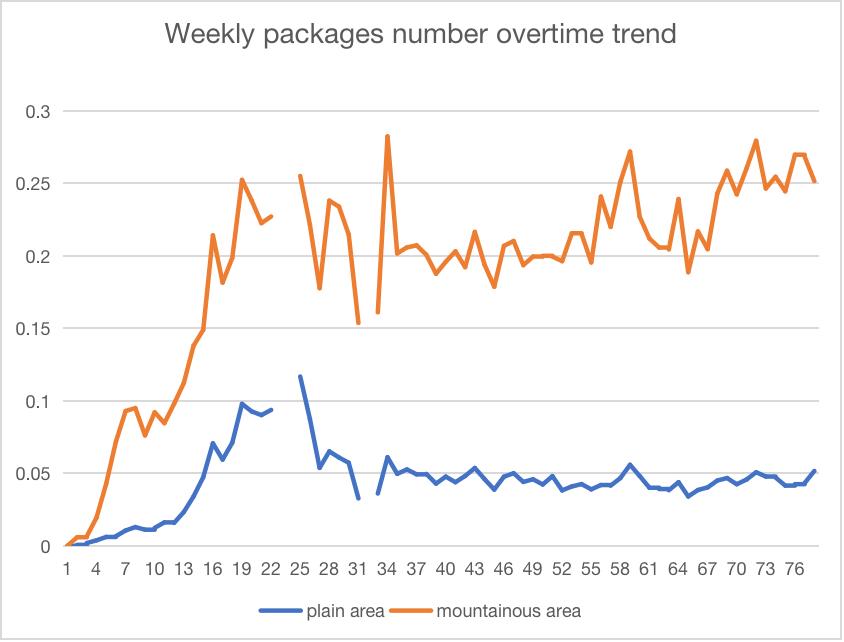
\includegraphics[width=5cm,height=4cm]{over-time.png}                                                                                         
\end{figure}                                             
\mbox{\hspace{2em}}
Apart from the average packages across time, the overtime trends of the weekly packages also attract us more. Here we show the average weekly packages of the delivery spots for mountainous area and plain area respectively. We can see from the graph that after the introduction of the delivery program, the weekly packages grow quickly, and reach a peak at approximately 25 weeks after\footnote{We drop week 23~24 and week 32 due to missing record of data.}. However, then the trends of the weekly packages diverge between the mountainous area and the plain area. The packages of the mountainous area maintains at a relatively high level, (although exit fluctuations.) But the packages quickly drop down and then maintains at a relatively low level in the plain area. This pattern in the plain area suggests that people make quick adjustments according to their past experience, and this learning process is relatively fast. After the number of packages reaches to a peak in around week 25, the packages number quickly fall and reaches a steady state in approximately 9 weeks. This fact may indicate that the demand for further logistics (or online shopping) in the plain area is lower than in the mountainous area.\\
\mbox{\hspace{2em}}
Motivated by these facts, we decide to look further into other geographical and demographical characteristics of each village. We focus on the average distance to the town center of each administrative village and try to give some explanations. Also, since the “bazaar culture” plays an important role in rural China, we further discuss the effect of local bazaars on rural logistics and e-commerce.\\
\subsection{Specification and variable construction}
To test for the effects of the distance to the town center on the average weekly packages number, we estimate the following equation:\\
\begin{equation*}
    \begin{aligned}
        & Package_i=\alpha+\beta distance_i+x_i'\gamma+\eta_{r}+\epsilon_i\\
    \end{aligned}
\end{equation*}
\mbox{\hspace{2em}}
Where $Package_i$ is the average weekly package number per household for an administrative village $i$. Since we don’t have the exact number of how many households adopt the new system, we just divide the weekly packages number by the whole household number of an administrative village. $distance_i$ is the average distance of an administrative village to the town center. $\beta$ is the coefficient of interest. $x_i$ is a vector of controls. In our preferred specification, this will include poverty rates (as a proxy for income), average distance to the delivery spots, average household numbers of the natural villages, how many delivery spots are there in administrative village $i$. $\eta_r$ is the dummy variable of whether administrative village $i$ is located in town $r$. (In case of collinearity, Mizhi town is omitted.) The construction and calculation of these variables are as follows:\\
{\bfseries Poverty rates:} We use the average poverty percentage of an administrative village as a proxy for income. This data comes from the records of the local government. Since the average income of Midu County is just above the poverty line and the average poverty percentage has a large variance among villages, poverty rate is a valid proxy for average income.\\
{\bfseries Average distance to the town center:} We measure the average distance to the town center of each administrative village, using the route recommended by Baidu Map. However, this distance is measured by minutes of car drive. Since the road conditions are quite different between the mountainous area and the plain area, we use minutes of car drive to represent the distance to town center to simulate the travel cost.\\
{\bfseries Average distance to the delivery spots:} For each administrative village, we calculate the distance from every natural village to the closest delivery spot. This is also measured using the route recommended by Baidu Map. We then average these distances by the population of natural village. Since for some of the natural villages are within a few minutes of walk to the delivery spots, and some of the natural villages are few kilometers away from the closest delivery spots, we can’t measure what kind of transportation do the villagers take to get to the delivery spots. So we just use the distance in kilometers recommended by Baidu Map.\\
{\bfseries Information about local bazaars:} We are also interested in how the local bazaar may affect the adoption of further logistics. And we put the dummy of whether there is a local bazaar locating in the administrative village in the main regression. The information about local bazaar comes from Midu annals (2005). There are 17 local bazaars in total. 8 of them locate in the eight town centers, while the other 9 bazaars locate in other 9 administrative village.\\
\subsection{Regression results and explanations:}
The main regression results are as follows:\\
% Table generated by Excel2LaTeX from sheet '工作表1'
\begin{longtable}{|l|r|r|r|}
    \toprule
    weekly average pacakges & \multicolumn{1}{l|}{coefficient} & \multicolumn{1}{l|}{sd} & \multicolumn{1}{l|}{p-value} \\
    \midrule
    \multicolumn{1}{|p{5.09em}|}{weekly average packages} & 0.2174 & 0.055 & 0.000  \\
    \midrule
    average distance to the city center (mins) & 0.0044 & 0.002 & 0.032 \\
    \midrule
    average distance to the delivery spots(km) & -0.0136 & 0.011 & 0.216 \\
    \midrule
    numbers of delivery spots of an administrative village & 0.0164 & 0.029 & 0.579 \\
    \midrule
    average number of households per natural village & 0.00014 & 0.0002 & 0.507 \\
    \midrule
    poverty rate & 0.1436 & 0.2789 & 0.609 \\
    \midrule
    deju  & 0.0697 & 0.1102 & 0.53 \\
    \midrule
    juli  & 0.0225 & 0.1042 & 0.83 \\
    \midrule
    niujie & 0.0523 & 0.1296 & 0.689 \\
    \midrule
    micheng & -0.0265 & 0.1108 & 0.812 \\
    \midrule
    yinjie & -0.0544 & 0.1143 & 0.636 \\
    \midrule
    xinjie & 0.00016 & 0.1275 & 0.999 \\
    \midrule
    hongyan & -0.0234 & 0.1171 & 0.843 \\
    \midrule
    \_cons & -0.0269 & 0.1424 & 0.851 \\
    \bottomrule
    \end{longtable}%

\mbox{\hspace{2em}}
We can see from the regression results that the average distance measured by minutes of car drive to the town center has a positive effect on the weekly packages per household of an administrative village. And this effect is statistically significant at the 0.05 level. Holding other variables constant, on average one minute closer to the town center will decrease the weekly packages number for 0.0043. (The minimum average weekly packages is 0.011, and the standard deviation is 0.183.) Although the coefficient of the average distance to the delivery spots is not statistically significant, the negative sign suggests that the packages is fewer for administrative village which on average is far from the delivery spots. It is worth noting that whether there is a bazaar locating in the administrative village significantly increase the number of packages. Holding other things constant, on average, administrative villages which have a bazaar located in have 0.213 more weekly packages than administrative villages without a bazaar. Average household number of an administrative village, poverty rates, and dummies of the towns are all statistically insignificant. In total, these variables can explain 57.14\% the variation of the weekly packages number per household. (The adjusted R square is 45.96\%.)\\
\mbox{\hspace{2em}}
Due to the data limitation, we can only give description of these correlation relationships, and couldn’t give the determination of causality. However, we still try to provide some explanations for these correlation relationships.\\
\mbox{\hspace{2em}}
Firstly, in the previous logistics system, since most of the logistics companies only deliver the packages to the town center, people have to go to the town to pick up their packages (for most of the time). After the introduction of rural logistics, whether the villagers choose to adopt it depends on their cost in two conditions. If their estimated cost to get to the town center (both travel cost and time cost) is smaller than the extra two yuan for the further delivery, then they will not choose to opt in. Thus, for villagers who live close to the town center, their willingness to pay maybe very low for the extra delivery and they will not choose to opt in. But for villagers who live far from the town center, it reduces their total cost for choosing the logistics, so their willingness to pay becomes much higher, especially in the mountainous area where transportation is inconvenient. As a result of the difference in willingness to pay, there may be more people choosing to adopt the rural logistics in the mountainous area, thus resulting in more packages in the remote area. \\
\mbox{\hspace{2em}}
We also raise another explanation of why there are more packages in the remote area: the substitution effect between the local market and online shopping. The varieties of goods are usually very limited in the villages, and the town center has a much higher variety. There are also big local bazaars located in the town center. For people living near to the town center, their accessibility to local market and varieties of goods are much higher than people living in remote places. Thus, the substitution effect between the local market and online shopping is stronger in places near the town center, and people in remote areas rely more on online shopping. If we have the exact number of people registering in the new logistics system for each delivery spot, we can distinguish between these two effects: Larger proportion of villagers registering in the remote area will suggest the first hypothesis of willingness pay, and more average packages per registered household will suggest the second hypothesis of the substitution effect between online and offline shopping.\\
\mbox{\hspace{2em}}
Next, we would like to discuss about the effect of local bazaars. The “bazaar culture” in rural China has a long history with thousands of years. A bazaar is a kind of big market or big fairs which only open on specific “bazaar days”. The opening frequency of a bazaar varies, some open twice a week or once a week, and some open once every four days. Once being set, the bazaar dates are seldom changed. The location, bazaar dates and the trading volume of a bazaar are required to be stated in the County Annals. On a bazaar day, pedlars from far or near all come together to the market place, and local residents usually go to the bazaar to purchase goods on a regular basis according to the bazaar dates. “The existence of the local bazaars greatly shapes the moving area of the local residents.”  As a result of the “bazaar culture”, villages with bazaars may serve as a kind of “vice center” of a town. The frequent gathering of people from other places may also speed up the spreading of information. As a result, people living close to the bazaar areas may have more information about the further logistics program, thus more people may choose to opt in. What’s more, since the villagers have the habit of regularly going to the bazaar to purchase goods, they can just pick up their packages by the way when going to the bazaar if their address of the delivery spots is near the bazaar place. So for villagers living near to a bazaar, their additional travel cost to the delivery spots will be eliminated since they are also going to the bazaar regularly. There are also chances that some villagers live far from the bazaar, but the distance to the closest delivery spots is still quite distant, they just change their delivery address into the bazaar place since they will go to the bazaar regularly anyway. It accordingly results in more packages in the delivery spots near the bazaar place.\\
\section{Cost-benefit analysis}
We conduct a simple cost-benefit analysis using the information from the logistics company. The cost of the logistics company can be divided into several parts: sorting fee of the workers, venue rental cost, gasoline cost and wages paid to the drivers. Since we don’t know how many workers do they employ for the sorting procedure and the venue rental cost, we just skip these two parts and focus mainly on the delivery cost. (Which includes the gasoline cost and wages for the drivers.) From the interview with the logistics company, we know that they send 8 lorries to 8 towns respectively to deliver the packages everyday. As stated above, We calculate the delivery cost as follows:\\
\begin{equation*}
    \begin{aligned}
        &C_{delivery}=L\times P_{gas}+wage\\
    \end{aligned}
\end{equation*}
\mbox{\hspace{2em}}
Where $L$ is the distance of a daily trip for each truck. We imitate the optimum routine for the drivers to get to all of the delivery spots of a town. Specifically, we calculate the minimum distance via all of the delivery spots using Baidu Map. $P_{gas}$  is the gasoline cost per kilometer. We estimate $P_{gas}$  as 1.245yuan/km. (We take the price of \#92 petrol as 8.3 yuan/L, and the petrol consumption of a 4.2 meters truck as 0.15 L/km. 8.3yuan/l * 0.15L/km = 1.245yuan/km.) Since we don’t know the wages of the drivers, we first use the average income of Midu county in 2020 as the wage of the drivers. (11981/12=998.4yuan/month ,998.4/30=33.3 yuan/trip) We then estimate two other cases of 50 yuan per trip and 100 yuan per trip. Because there has been big changes in the revocation of the delivery spots in Mizhi town, and Mizhi is also the smallest town of Midu county, we just skip Mizhi town and conduct the cost-benefit analysis on the other 7 towns.\\
\mbox{\hspace{2em}}
For the income part, since the company charge 2 yuan per package for most of the delivery spots, we just take 2 yuan for all of the delivery spots for simplification. We then investigate three conditions of the share proportion between the logistics company and the agents: 50\%:50\%, 60\%:40\% and 70\%:30\%. (The share proportion used to be 60\%:40\%, but now the share proportion is 50\%:50\%.) So the revenue of the company is 1 yuan per package under the share proportion of 50\%:50\%, 1.2 yuan per package under 60\%:40\% and 1.4 under 70\%:30\%. We also look into the condition where there are no shares for the agents.\\
\mbox{\hspace{2em}}
The results are as follows: \\
\begin{tabular}{|p{5.09em}|l|l|l|l|l|l|l|l|}
    \toprule
    Town  & \multicolumn{1}{p{3.06em}|}{Niujie} & \multicolumn{1}{p{3.06em}|}{Deju} & \multicolumn{1}{p{2.825em}|}{Juli} & \multicolumn{1}{p{3.12em}|}{Yinjie} & \multicolumn{1}{p{3.09em}|}{Micheng} & \multicolumn{1}{p{3.235em}|}{Xinjie} & \multicolumn{1}{p{3.175em}|}{Hongyan} & \multicolumn{1}{p{3.56em}|}{Total} \\
    \midrule
    Cost: (yuan) &       &       &       &       &       &       &       &  \\
    \midrule
    gasoline cost per week & 2383.5525 & 1723.1298 & 1085.889 & 718.9875 & 932.9404 & 356.4435 & 533.0094 & 7733.9521 \\
    \midrule
    gasoline cost per week+ driver's wage (33.3yuan*7 days) & 2616.6525 & 1956.2298 & 1318.989 & 952.0875 & 1166.0404 & 589.5435 & 766.1094 & 9365.6521 \\
    \midrule
    gasoline cost per week+ driver's wage (50yuan*7days) & 2733.5525 & 2073.1298 & 1435.889 & 1068.9875 & 1282.9404 & 706.4435 & 883.0094 & 10183.9521 \\
    \midrule
    gasoline cost per day + driver's wage (100yuan*7 days) & 3083.5525 & 2423.1298 & 1785.889 & 1418.9875 & 1632.9404 & 1056.4435 & 1233.0094 & 12633.9521 \\
    \bottomrule
    \end{tabular}%
 

\begin{tabular}{|p{5.09em}|l|l|l|l|l|l|l|l|}
    \toprule
    Revenue: (yuan) &       &       &       &       &       &       &       &  \\
    \midrule
    total weekly package number & 1146.24 & 1833.65 & 635.1 & 500.66 & 1092.05 & 475.43 & 324.79 & 6007.92 \\
    \midrule
    revenue under 50\%:50\% (per week) & 1146.24 & 1833.65 & 635.1 & 500.66 & 1092.05 & 475.43 & 324.79 & 6007.92 \\
    \midrule
    revenue under 60\%:40\% (per week) & 1375.488 & 2200.38 & 762.12 & 600.792 & 1310.46 & 570.516 & 389.748 & 7209.504 \\
    \midrule
    revenue under 70\%:30\% (per week) & 1604.736 & 2567.11 & 889.14 & 700.924 & 1528.87 & 665.602 & 454.706 & 8411.088 \\
    \midrule
    revenue with no shares for the agents & 2292.48 & 3667.3 & 1270.2 & 1001.32 & 2184.1 & 950.86 & 649.58 & 12015.84 \\
    \bottomrule
    \end{tabular}%
    
    
\mbox{\hspace{2em}} 
From the cost-benefit analysis, we can see that under the share proportion of 60\%:40\% and 50\%:50, this kind of business mode is definitely not profitable for the company, even if we skip the sorting fee for the workers and the venue rental charge. Under the share of 70\%:30\%, the revenue from the further delivery can just cover the petrol cost. However, if the company doesn’t pay any shares of income to the agents, the revenue from the further delivery can cover the costs if the driver’s wage is 33.3 yuan per trip or 50 yuan per trip. But they can’t break even if the driver’s wage is 100 yuan per trip. The results from this cost-benefit analysis coincide with the evidence that the logistics company was at a loss in the past 2 years and had to rely on the subsidy from the local government. \\
\mbox{\hspace{2em}}
These results inspire us to think about why the company choose to maintain such a high share proportion with the agents. From the interview with the company managers, we know that the agents are usually shop owners in the villages. In fact, the company wants to build new delivery spots in some villages that are remote but have a relative large population, however they couldn’t find anyone who are willing to serve as an agent there. The high share proportion also indicates that there are few people willing to become an agent. Actually, for the agents, they are not responsible for the delivery process and the share proportion of the revenue is pure profit for them. So why there are few people willing to become agents? We further know that the agents need to be responsible for the process of “recording”. This is a kind of standardized operation when the express packages are escorted to the last delivery spot of the whole delivery process. The recording procedure usually needs a professional bar-code scanner and the agents should learn how to use it. We guess that this procedure of technology adoption adds a barrier to the shop owners which may reduce their willing to become the agents. What’s more, the agents are also responsible for taking care of the packages from being lost or stolen. These responsibilities add extra time cost to the agents. The technology adoption barriers and other responsibilities makes the number of potential agents smaller. This endows the local shop owners more bargaining power when negotiating with the logistics company.\\
\mbox{\hspace{2em}}
From the interview with the company and a local agent, we get to know that there are actually other companies planning to provide further delivery, which may form competition to some extent. (for example, a company called Hope logistics is planning to provide further delivery in Midu county.) However, the smart rural logistics center is still the biggest monopolist in Midu right now. But even given the condition of no competitors, restricted with the willingness to pay of local residents and the bargaining power of the agents, it is still hard for them to make profits. From the information of the delivery spots, we can see that the logistics company pay more attention to the plain area: For some administrative villages, they build two or three delivery spots. But for the mountainous area, they at most build one delivery spot for an administrative village. Combining with our discussion about the difference of willingness to pay between the plain areas and the mountainous areas, maybe the logistics company can establish more delivery spots in the mountainous area to cover more people. There are many natural villages that are still far away from the delivery spot in the administrative village in the mountainous area. If the company can build more delivery spots in these village, they may earn more given the relative high willingness to pay of these villagers.\\
\mbox{\hspace{2em}}
In this cost-benefit analysis, we didn’t take the outward logistics part into account. After the construction of the delivery spots and further logistics system, adding outward delivery service can be zero cost for the logistics company. The company can also charge higher fee for outward delivery. With the fast development of rural e-commerce, the quantity of outward transportation (especially the outward transportation of agricultural goods) shouldn’t be neglected. Although the logistics companies are not earning money right now, this industry may be quite profitable in the near future.\\
\section{Conclusion:}
This article studies how people react when the rural logistics system specifies to the village level. We regard an administrative village as an unit, and we discover that weekly packages per household vary greatly among administrative villages. We then look into the relationship between the geography conditions and the average weekly packages of each administrative village. Specifically, we find that the average weekly packages of villages in the mountainous area is much more than villages in the plain area. (Despite people’s income is lower and villages are more dispersed in the mountainous area.) Moreover, after the introduction of further logistics, people adopt quickly and reach the peak in a few months of time. However, the weekly packages mode then diverges between the mountainous area and the plain area: it remains at a high level in the mountainous area, while it quickly drops down and retains at a low level in the plain area. This change reflects people’s learning process from their past experience, and this process is quite swift. The two patterns also indicate that the demand for further logistics in the plain area isn’t as large as in the mountainous area. We then look further into the average distance to the town center of each administrative village. We find that the average distance to the town center can explain 42\% of the variance of the weekly packages (adjusted R square is 0.27). (Further the distance, more the packages.) On this basis, we look into whether local fairs are located in the administrative village has an impact. We find that having a local fair in the village will significantly increase the weekly package number of the administrative village, and this raise R square from 0.42 to 0.58 (adjusted R square is 0.46). In our regression, the effect of the poverty percentage of an administrative village isn’t statistically significant. The average distance to the delivery spot of an administrative village is also insignificant.\\
\mbox{\hspace{2em}}
Due to the limitation of data, we only give a description of these phenomena, and we couldn’t give the determination of causality. However, we put forward some possible explanation of these phenomena. First, for people living close to the town center, or in the plain area where transportation is more convenient, their willingness to pay for this further delivery isn’t very high, so there is no need for these people to choose to opt in this further delivery. It’s also possible that people living in the plain area or close to the town center have higher access to the local markets, (where variety of goods is much higher than small shops in the villages.) so their demand for online shopping is not as much. While for people living in the mountainous area, it will take them more transportation cost (and time cost) to go to the town center and local markets. These factors above mays make people in the mountainous areas rely more on online shopping. If we have further statistics on the number of people who adopt to this further delivery for each delivery spot, perhaps we can distinguish these two effects. For administrative villages that have big fairs locating in, since people in rural places of China is accustomed to going to the fairs regularly, their time to pick up packages and go to the fairs can match well, so the existence of the local fairs cuts the extra cost for people getting to the delivery spots. It’s beneficial for them to choose online shopping without extra cost and can enjoy the varieties of goods. Additionally, maybe the information fluidity is higher in places with local fairs, so more people are exposed to the information about the new establishment of the delivery spots, thus there are more people adopting this further delivery.\\
\mbox{\hspace{2em}}
Finally, we conduct the cost-benefit analysis. The result shows that, when only considering the gasoline expense and the drivers’ wages, under the share proportion of 50\%:50\% between the company and the agents, it is hard for the company to break even. However, if the share proportion is changed into 60\%:40\%, the company can roughly break even when only considering the gasoline expense and the drivers’ wages. The reason why the company has to maintain a high share proportion with the agents is that the size of potential agents is quite small. In this way, the agents have relatively larger bargaining power. From the cost-benefit analysis, we can see that the rural logistics industry is quite harsh in the present situation. It is hard for the logistics company to get self-financed without the subsidy from the local government. Nevertheless, the establishment of further logistics system is still of great significance. Not only can the further logistics system improve welfare of local residents, but also lays a foundation for outward transportation of agricultural goods. With the fast development of rural e-commerce, the quantity of outward transportation shouldn’t be neglected. Although the logistics companies are not earning money right now, this industry may be quite profitable in the near future.\\
{\bfseries\sihao Reference}
Ran, J. (2017, September). Research on the Relationship between Logistics Development and Consumption of Rural Residents. In {\it 2nd International Conference on Judicial, Administrative and Humanitarian Problems of State Structures and Economic Subjects (JAHP 2017)} (pp. 184-188). Atlantis Press.\\
Jacoby, H. G. (2000). Access to markets and the benefits of rural roads. {\it The economic journal, 110(465)}, 713-737.\\
Tu, C., He, M., Ren, Y., \& Qin, Y. (2018). Research on the Logistics Embeddedness in Rural Town E-commerce. In {\it Proceedings of the Fifth International Forum on Decision Sciences} (pp. 241-254). Springer, Singapore.\\
Liu, W. (2020). Route optimization for last-mile distribution of rural E-commerce logistics based on ant colony optimization. {\it IEEE Access}, 8, 12179-12187.\\
Yang, F., Dai, Y., \& Ma, Z. J. (2020). A cooperative rich vehicle routing problem in the last-mile logistics industry in rural areas. {\it Transportation Research Part E: Logistics and Transportation Review, 141}, 102024.\\
Giuffrida, M., Mangiaracina, R., Perego, A., \& Tumino, A. (2017). Cross-border B2C e-commerce to Greater China and the role of logistics: a literature review. {\it International Journal of Physical Distribution \& Logistics Management.}\\
Jalali, A. A., Okhovvat, M. R., \& Okhovvat, M. (2011). A new applicable model of Iran rural e-commerce development. {\it Procedia Computer Science, 3}, 1157-1163.\\
Rhodes, J. (2009). A strategic framework for rural micro-enterprise development: The integration of information communication technology (ICT), e-commerce, marketing, and actor-network theory. {\it Perspectives on global development and technology, 8}(1), 48-69.\\
Zhang, Y., Zhang, Y., Li, Y., Liu, S., \& Yang, J. (2017). A study of rural logistics center location based on intuitionistic fuzzy TOPSIS. {\it Mathematical Problems in Engineering, 2017}.\\
Couture, V., Faber, B., Gu, Y., \& Liu, L. (2021). Connecting the countryside via e-commerce: evidence from China. {\it American Economic Review: Insights, 3}(1), 35-50.\\
Gong, X. (2019). Coupling coordinated development model of urban-rural logistics and empirical study. {\it Mathematical Problems in Engineering, 2019}.\\
Cárdenas, I., Beckers, J., \& Vanelslander, T. (2017). E-commerce last-mile in Belgium: Developing an external cost delivery index. {\it Research in transportation business \& management, 24}, 123-129.
Feng, Z. (2020). Constructing rural e-commerce logistics model based on ant colony algorithm and artificial intelligence method.{\it Soft Computing}, 24(11), 7937-7946.\\
Qu, L., \& Dai, Y. (2021, February). Research on the path of improving the service quality of rural E-commerce logistics in Jilin province based on computer. In {\it Journal of Physics: Conference Series} (Vol. 1744, No. 3, p. 032144). IOP Publishing.\\
Kshetri, N. (2018). Rural e-commerce in developing countries. {\it It Professional, 20(2)}, 91-95.\\
Cui, M., Pan, S. L., Newell, S., \& Cui, L. (2017). Strategy, resource orchestration and e-commerce enabled social innovation in Rural China. {\it The Journal of Strategic Information Systems, 26}(1), 3-21.\\
Liu, M., Min, S., Ma, W., \& Liu, T. (2021). The adoption and impact of E-commerce in rural China: Application of an endogenous switching regression model. {\it Journal of Rural Studies, 83}, 106-116.\\
Chen, X., \& Zhou, J. (2011, June). The Research on the Interaction Effects of Rural Logistics and Economic Development. In {\it ICEIS (2)} (pp. 167-171).\\
Jiang, X., Wang, H., Guo, X., \& Gong, X. (2019). Using the FAHP, ISM, and MICMAC approaches to study the sustainability influencing factors of the last mile delivery of rural E-commerce logistics. {\it Sustainability, 11}(14), 3937.\\


  




























\end{document}